\documentclass[]{BasiliskReportMemo}
\usepackage{AVS}


\newcommand{\submiterInstitute}{Autonomous Vehicle Simulation (AVS) Laboratory,\\ University of Colorado}

\newcommand{\ModuleName}{thrMomentumDumping}
\newcommand{\subject}{Thrusting Firing Module to Cycle Through the RW Momentum Dumping}
\newcommand{\status}{initial document draft}
\newcommand{\preparer}{H. Schaub}
\newcommand{\summary}{This module reads in the desired impulse that each thruster must produce to create inertial momentum change to despin the RWs.   The output of the module is a setof of thruster firing times.  Each thruster can only fire for a maximum time that matches a single control period.  After this the thrusters are off for an integer number of control periods to let the RW re-stabilize the attitude about an inertial pointing scenario.    }


\begin{document}


\makeCover


%
%	enter the revision documentation here
%	to add more lines, copy the table entry and the \hline, and paste after the current entry.
%
\pagestyle{empty}
{\renewcommand{\arraystretch}{1.1}
\noindent
\begin{longtable}{|p{0.5in}|p{4.5in}|p{1.14in}|}
\hline
{\bfseries Rev}: & {\bfseries Change Description} & {\bfseries By} \\
\hline
Draft & Initial document creation & H. Schaub \\
\hline

\end{longtable}
}

\newpage
\setcounter{page}{1}
\pagestyle{fancy}

\tableofcontents
~\\ \hrule ~\\

\begin{figure}[htb]
	\centerline{
	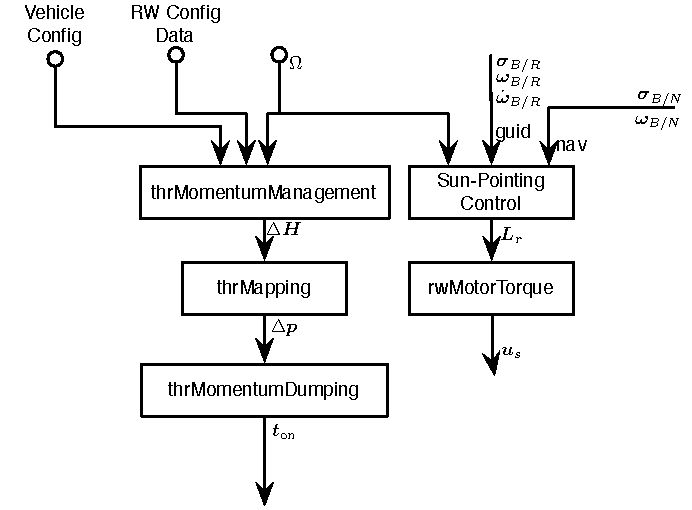
\includegraphics[]{Figures/rwMomentumOverview}
	}
	\caption{Overview of the Modules Used to Perform Reaction Wheel Angular Momentum Dumping.}
	\label{fig:Fig1}
\end{figure}

\section{Introduction}
To manage the Reaction Wheel (RW) angular momentum build-up over time, a thruster-based momentum dumping strategy is used.  Figure~\ref{fig:Fig1} illustrates how the momentum dumping will occur simultaneously with an inertial pointing control solution.  Assume the spacecraft contains $N_{\text{RW}}$ RWs, and $M_{\text{thr}}$ thrusters.   The momentum dumping management module already evaluated the required $\leftexp{B}{\Delta}\bm H$ that must be achieved in this round of momentum dumping.  The spacecraft is assumed to be held inertially fixed, such as in sun-pointing.  



\begin{figure}[t]
	\centerline{
	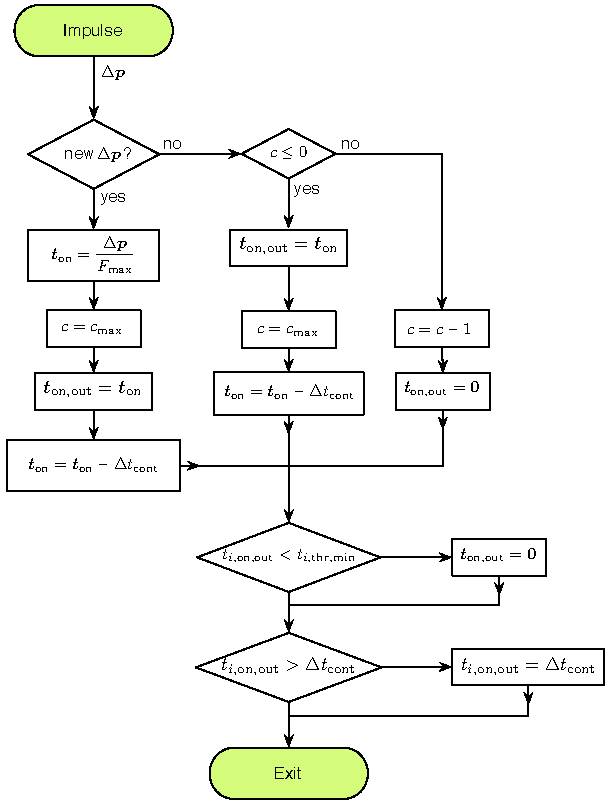
\includegraphics[]{Figures/rwMomentumDumping}
	}
	\caption{Overview of the Reaction Wheel Angular Momentum Dumping Module.}
	\label{fig:Fig2}
\end{figure}


\section{{\tt thrMomentumDumping} Module Description}
This modules receives the vector of thruster impulses $\Delta\bm p$ from a thruster mapping module.  It first checks to see if this $\Delta\bm p$ is new.  If yes, it compute the overall thruster on-times through
\begin{equation}
	\bm t_{i,\text{on}} = \frac{\Delta \bm p}{F_{i,\text{max}}}
\end{equation}
where $F_{i,\text{max}}$ is the maximum thrust force achievable with the on-off type thruster.  This on-times are copied to the output thruster on times, and the thruster cycling counter is reset.  

If the $\Delta\bm p$ message is not new, then the counter flag is checked.  If the counter is strictly positive, the thrusters should be off to allow for the RW to stabilize the orientation.  In this case the output thruster times are set to zero, and the counter is decremented, and the remaining required thruster on-times are decremented by the control time period.

If the counter flag reaches zero it is time to fire the required thrusters again to implement the next chunk of the required thruster impulse.  The output thrust on times are set to the remaining thruster on times, the counter is reset, and the remaining thruster on times is decremented again by the control period.

Finally, the thruster on times are checked to be greater than the thruster minimum firing time, or the output time is set to zero.  Similarly, if the required thruster on time is larger than a control period, the thruster on time is set equal to the control period.  This ensures that the thrusters will fire for a single control period duration only before returning to an off-mode.  



\section{Module Parameters}
\subsection{{\tt maxCounterValue} Parameter}
This parameter dictates the number of control periods where the thrusters cycle off to allow the RWs to re-stabilize the orientation.  It must be set to a strictly positive value.  

\subsection{{\tt thrMinFireTime} Parameter}
This parameter determines what the minimum thruster firing time is, provided in units of seconds.  




\end{document}
